\documentclass{beamer}

\usepackage[utf8]{inputenc}


\title{Industry Advance}
\author{Davids Paskevics, Phillip Wellner, Alexander Berthold}
\institute{FU Berlin}
\date{2020}



\begin{document}

\frame{\titlepage}

\begin{frame}
	\frametitle{The project}
	\begin{itemize}
		\item Game for the GBA console \begin{itemize}
			      \item Got idea @spline last year
		      \end{itemize}
		\item Port/clone of the libre Java game \emph{Mindustry}
		\item Mashup of logistics sim/tower defense
		\item Wave-based gameplay good fit for portable gaming
	\end{itemize}
\end{frame}

\begin{frame}
	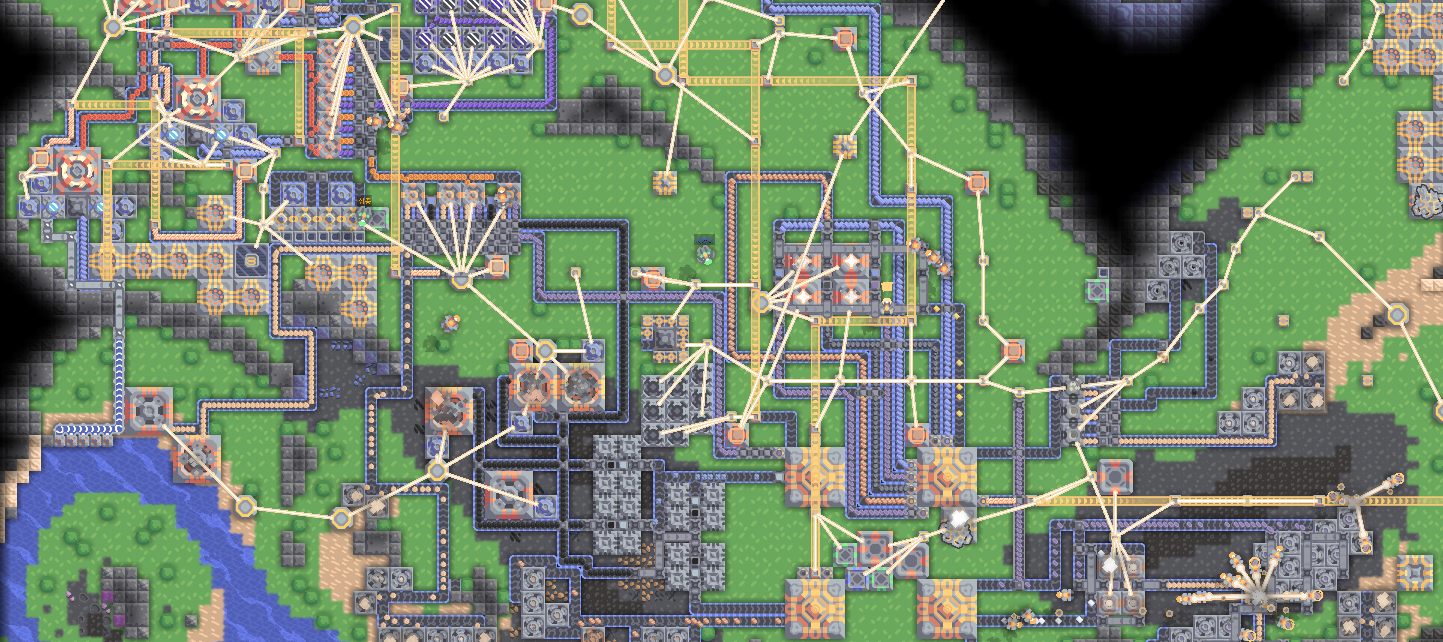
\includegraphics[scale=0.4]{images/mindustry.png}
\end{frame}

\begin{frame}
	\frametitle{Demo}
\end{frame}



\begin{frame}
	\frametitle{The hardware}
	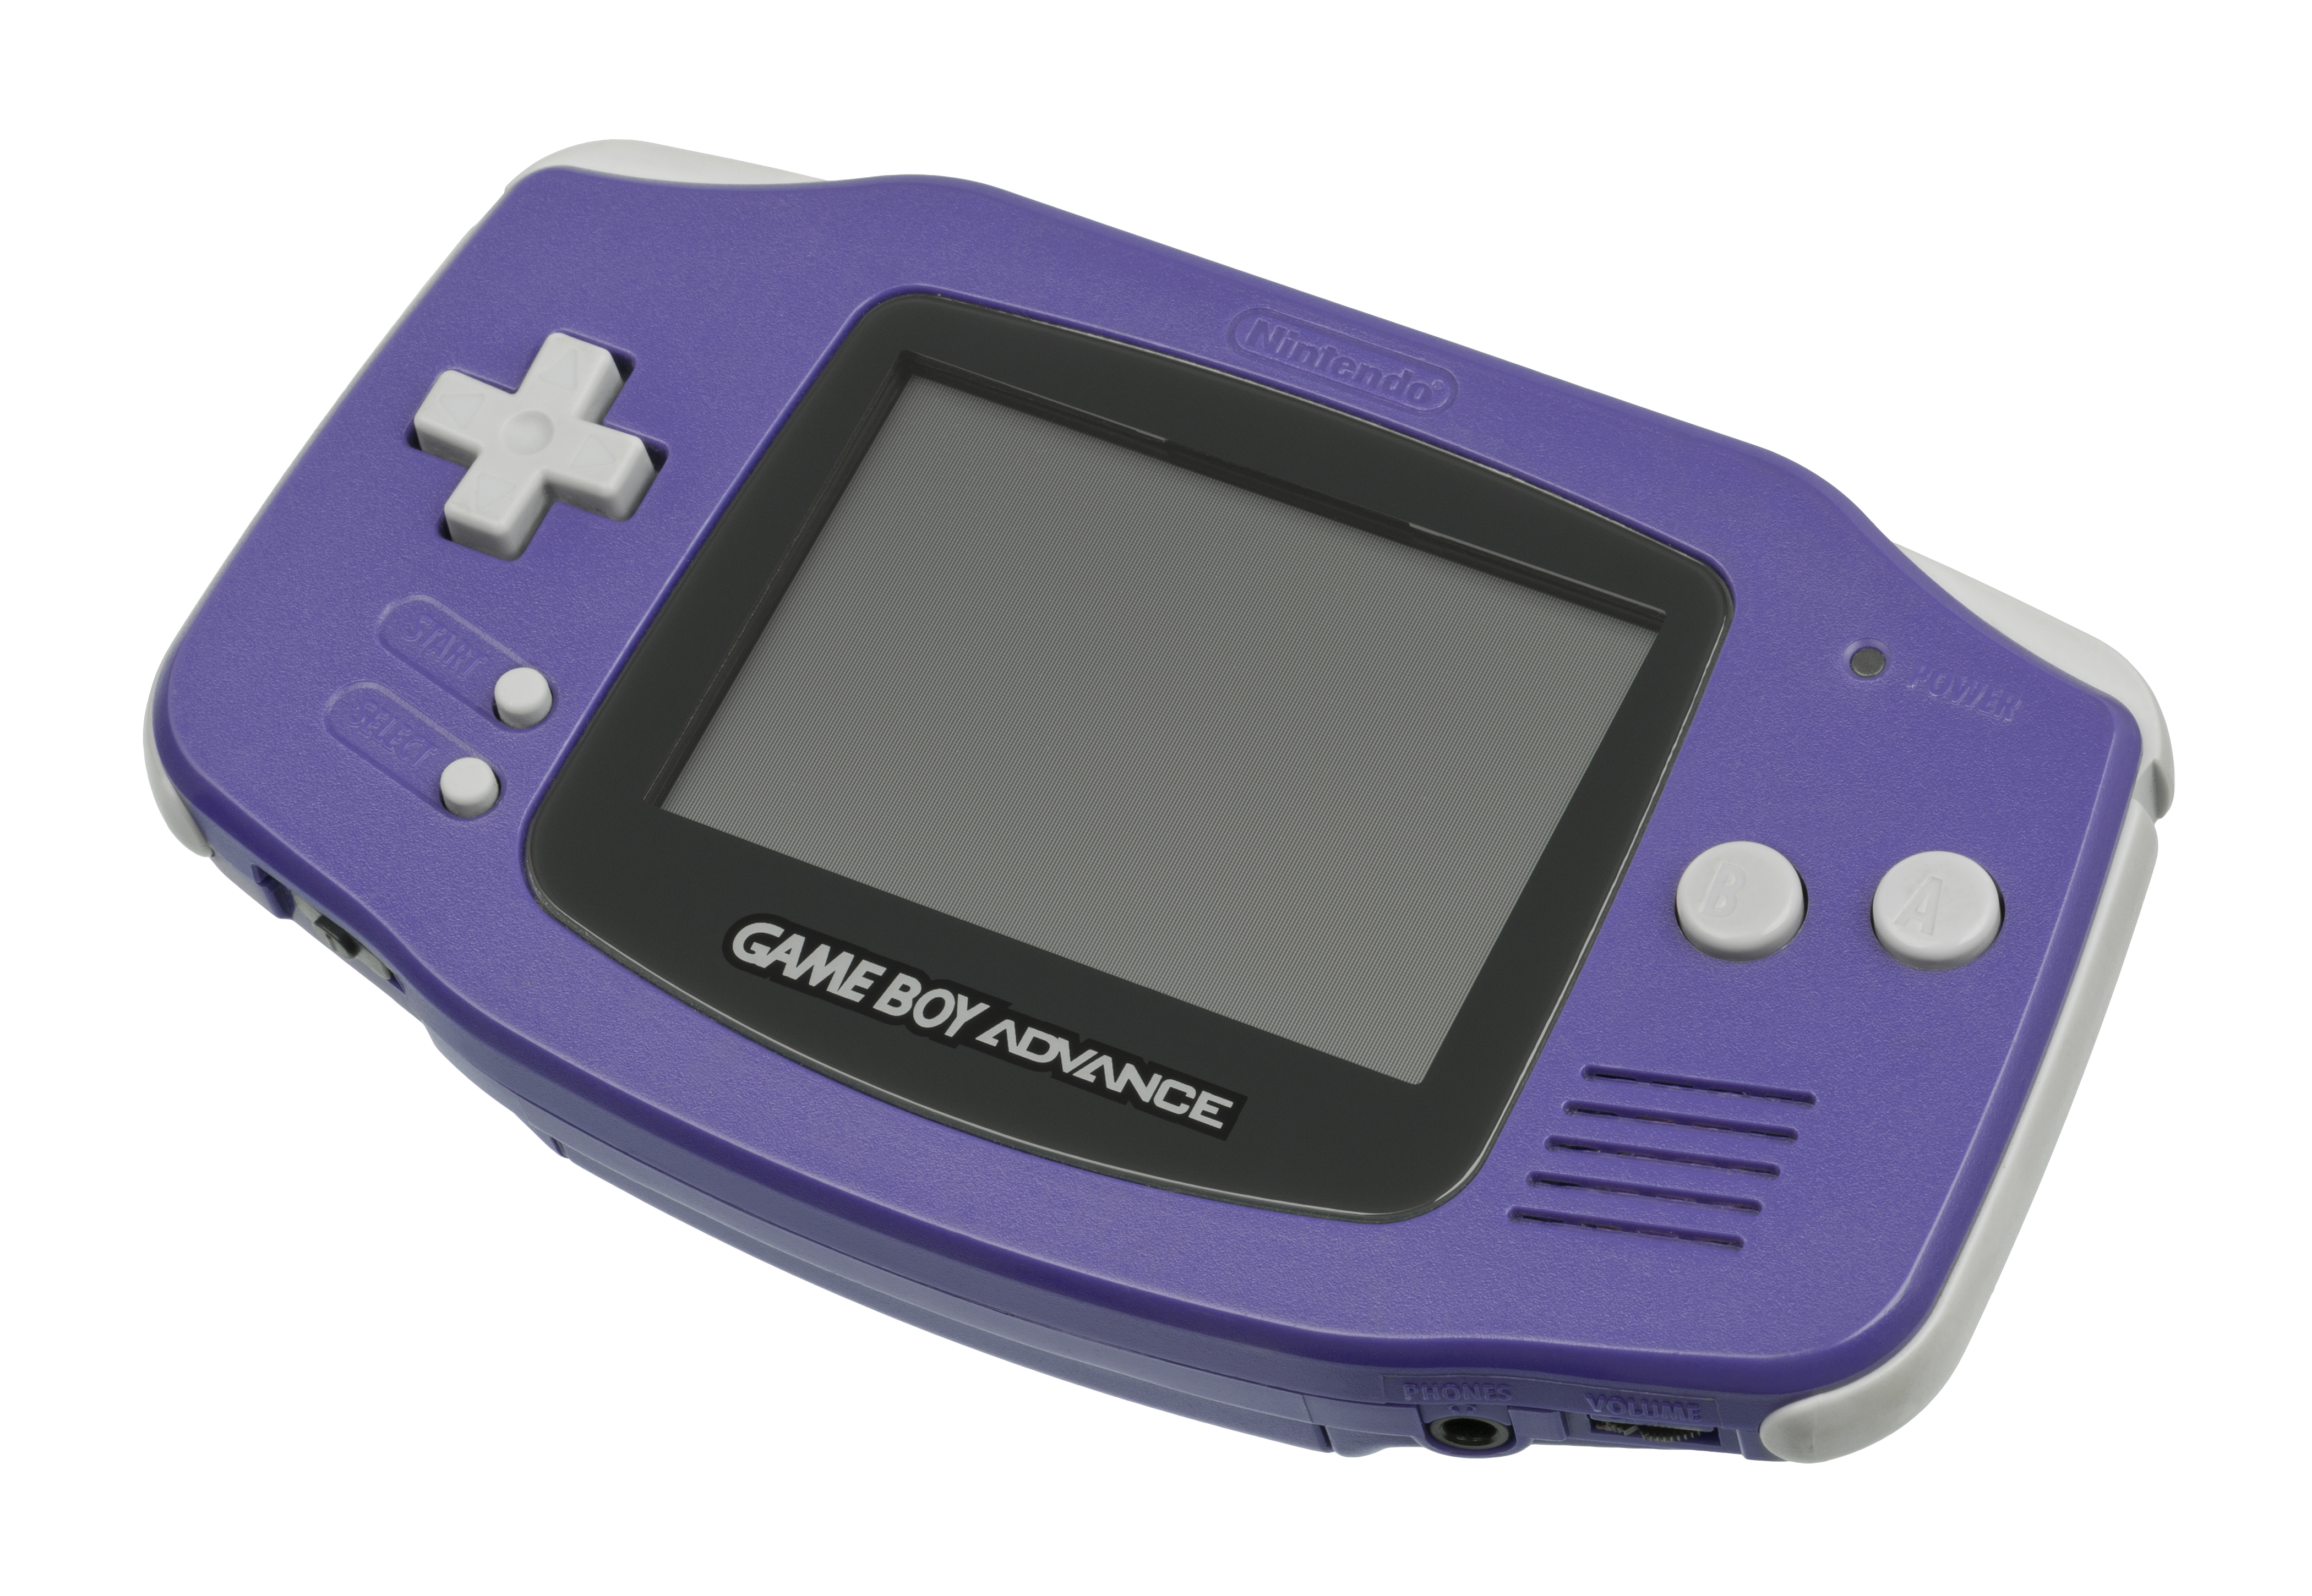
\includegraphics[scale=0.28]{images/Nintendo-Game-Boy-Advance-Purple-FL.jpg}
\end{frame}

\begin{frame}
	\frametitle{The hardware}
	\begin{itemize}
		\item Handheld game console by Nintendo
		\item JP release in 2000
		\item Engineered for cost and battery life \begin{itemize}
			      \item No OS, just BIOS
			      \item 32 bit ARMv4t ISA processor
			      \item Clock @16MHz
			      \item No cache
			      \item 32KiB fast (on-die) RAM $\xrightarrow[]{}$ We put stack here
			      \item 256Kib slow (off-die) RAM = narrow bus + wait cycles $\xrightarrow[]{}$ We put heap here
			      \item Up to 32MiB cart ROM
			      \item Nintendo wanted to make the "ultimate 2D handheld" $\xrightarrow[]{}$ no HW 3D support, FPU or division
		      \end{itemize}
	\end{itemize}
\end{frame}

\begin{frame}
	\frametitle{Prior art}
	\begin{itemize}
		\item ISA supported in \emph{LLVM} (and therefore \emph{rustc})
		\item Cross-compiling \emph{libcore} easy thanks to \emph{build-std} cargo feature
		\item rust-console/gba crate provides basic HAL
		\item Snake game from around 2015, but no "complex" games written in Rust to our knowledge
	\end{itemize}
\end{frame}

\begin{frame}
	\frametitle{Starting out}
	\begin{itemize}
		\item "Hello world" is tricky
		\item Easier to draw something
		\item Shouldn't be hard, right?
		\item Until you want to draw something useful for a game, that is
	\end{itemize}
\end{frame}

\begin{frame}
	\frametitle{Graphics on the GBA}
	\begin{itemize}
		\item Modern consoles/PCs are powerful enough to allow uploading pixels to the display freely
		\item GBA has such "bitmap" modes as well (slow!)
		\item Also supports HW accelerated "tile modes" (fast!)
		\item Custom GFX format, needs a converter \begin{itemize}
			      \item \emph{grit} most commonly-used homebrew tool, docs are meh
		      \end{itemize}
		\item All this makes custom engine a requirement:
	\end{itemize}
\end{frame}

\begin{frame}
	\frametitle{Graphics on the GBA}
	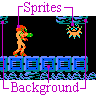
\includegraphics[scale=2.0]{images/tile_gfx_render.png}
\end{frame}

\begin{frame}
	\frametitle{Graphics on the GBA}
	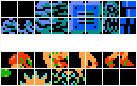
\includegraphics[scale=2.0]{images/tile_gfx_tileset.png}
\end{frame}

\begin{frame}
	\frametitle{We implemented}
	\begin{itemize}
		\item Not much gameplay (just movement, placing blocks, inventory system)
		\item But lots of engine work: \begin{itemize}
			      \item Sprite allocator with refcounting
			      \item Simple heap allocator
			      \item Support for maps of arbitrary size
			      \item Text engine
			      \item Filesystem (GBFS)
			      \item Various debug facilities (logging macro, debugger config)
			      \item Test framework
			      \item Map converter (WIP)
		      \end{itemize}
	\end{itemize}
\end{frame}

\begin{frame}
	\frametitle{We didn't finish}
	\begin{itemize}
		\item Picked a project too ambitious in scope
		\item Underestimated engine dev effort
		\item Underestimated effort needed for asset pipeline \begin{itemize}
			      \item Undocumented Mindustry save format (basically java classes dumped to disk)
			      \item Source of many bugs
			      \item Spent $>25\%$ of dev time there
		      \end{itemize}
		\item Project management failures (deadlines, working independently)
		\item Good ol' procrastination
		\item However, none of these issues were caused by Rust
		\item In fact, Rust helped speed up dev
	\end{itemize}
\end{frame}

\begin{frame}
	\frametitle{Some of our bugs}
	\begin{itemize}
		\item Grit is the devil!
	\end{itemize}
	\vskip 1em
	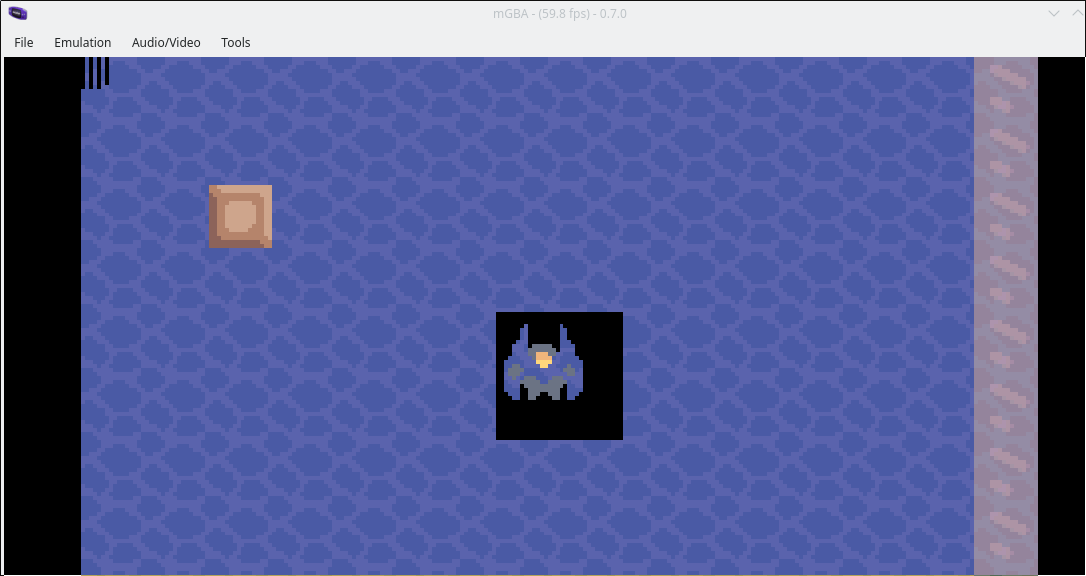
\includegraphics[scale=0.3]{images/grit_bug.png}
\end{frame}


\begin{frame}
	\frametitle{Rust ecosystem}
	\begin{itemize}
		\item Many easily integrated \emph{no\_std} crates
		      \begin{itemize}
			      \item \emph{serde} for map metadata loading from JSON
			      \item \emph{tiny\_ecs} for ECS (good pattern for structuring games in Rust)
			      \item \emph{hashbrown} for hashmap
			      \item \emph{fixed} for fixed-point maths (fast!)
			      \item Many more small ones used (\emph{arraystring}, \emph{array\_vec}, \emph{ansi\_rgb})
		      \end{itemize}
		\item Crates reduced dev time by a lot
		\item However: \begin{itemize}
			      \item Downside: Some assume stuff (atomics support)
			      \item Downside: Others are needlessly \emph{std}-dependent (made patches)
		      \end{itemize}

	\end{itemize}
\end{frame}

\begin{frame}
	\frametitle{Rust APIs/tooling}
	\begin{itemize}
		\item Tile-based custom text output w/ formatting in $<50$ LOC thanks to \emph{Write} trait
		\item Custom test framework w/ minimal boilerplate
	\end{itemize}
\end{frame}

\begin{frame}
	\frametitle{Rust safety}
	\begin{itemize}
		\item Only hit memory bugs in our \emph{unsafe} allocator
		\item Saves us a lot of time (which we need to squash logic bugs instead)
		% \item Could make more use of borrow checker for managing HW resources \begin{itemize}
		%	      \item Especially palette/tile/bg mgmt could be improved
			%\end{itemize}
	\end{itemize}
\end{frame}

\begin{frame}
	\frametitle{Rust speed}
	\begin{itemize}
		\item No CPU bottleneck yet, despite many abstractions
		\item Code isn't very optimized
		\item \emph{const\_fn} allowed for a low-RAM FS parser implementation
		\item Easy mixing of ARM/Thumb code would be nice (bus width)
	\end{itemize}
\end{frame}

\begin{frame}
	\frametitle{Conclusion}
	\begin{itemize}
		\item Surprisingly few Rust-related issues despite exotic target
		\item Will develop project further
		\item Interested? Fork us on github: https://github.com/industry-advance/industry-advance (take a look under "Projects" for roadmap!)
	\end{itemize}
\end{frame}



\end{document}
